\section{Introduction}

  The BBC is now over 100 years old (BBC, 2022) and is well known for it's TV channels and radio stations that are broadcast over the airwaves (Pilnick, Baer, 1973, p.3) 
  to peoples homes across the UK. However this old way of broadcasting, sending out airwaves on a certain frequency to an antenna, is becoming 
  less popular in the modern age of the internet. A study done by Ofcom showed that people
  \textit{'watched on average about 16\% less broadcast TV between 2019 ... and 2022'}, with viewing \textit{'decreasing by 47\%'} (Ofcom, 2023, p.7) between ages
  16-24. In addition another study carried out by media analyst firm Ampere found that in 2021 37\% of people claimed to watch no linear TV,
  this increased to 45\% by 2023 (Ampere Analysis, 2023).
  
  This fall correlates with the significant rise in internet enabled TVs in the home, with statista finding that 
  \textit{'In 2014 just 11 percent of households in the UK owned a Smart TV, whereas, in 2023, nearly 74 percent of households reported owning a Smart TV.'} (Statista, 2023).

  \begin{figure}[H]
    \centering
    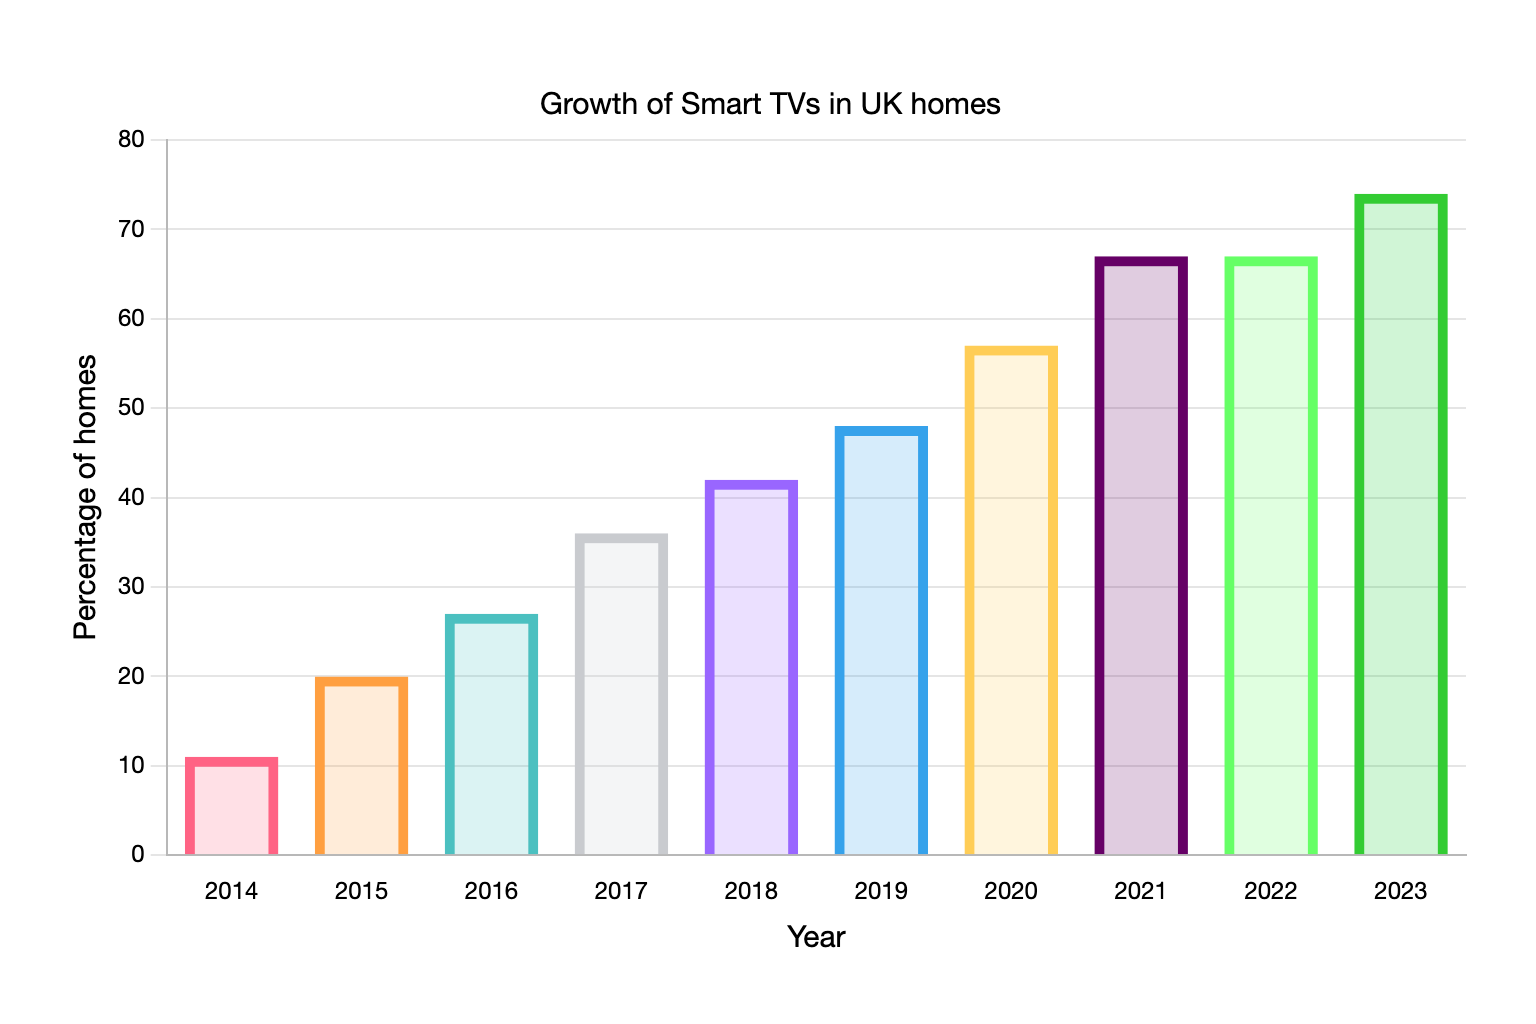
\includegraphics[width=6cm]{assets/smartTvGrowth.png}
    \caption{Bar chart showing growth of smart TVs in UK homes (Statista, 2023) \textit{Created with Line Graph Maker} (Line Graph Maker, 2023)}
    \label{fig:smartTvGrowth}
  \end{figure}

  Some of these devices still support OTA broadcasts, however devices like the Amazon Fire TV stick and Googles Chromecast, are purely internet
  based; However they do offer a \textit{'guide/epg'} section with Amazon having a development guide (Amazon, 2021) on how to integrate with it.
  Director general of the BBC, Tim Davie, in 2022 stated:
    \begin{quote}
      \textit{'The vision is simple: from today we are going to move decisively to  a digital-first BBC'} (Davie, 2022)
    \end{quote}

  This statement highlights the goal to put more organisational focus on these new forms of media and internet enabled devices. 
  
  This report will discuss an upgrade carried out to the BBCs \textit{'off-product'} schedules system, responsible for delivering up to date schedules to
  partners such as Freeview, Amazon and more. First I will give some background on the project, where I will discuss topics including storage Solutions
  and how they can work in parallel/multi-threaded systems, and strategies to protect live code systems in a CI/CD environment. I will also give some 
  background on the starting architecture of the system and how the changes align with the BBCs and teams OKRs (Sparks, 2024).
  
  Following that, I will discuss the work that was done. This will be broken down into 5 sections that align with our teams ways of working flow.
  \begin{enumerate}
    \item Requirements and epic creation
    \item Investigation and Spike
    \item Slicing and task/ticket creation
    \item Development of software
    \item Releasing of software
  \end{enumerate}

  I will then talk about the outputs of the project. Theses will include burn-up charts for the projects, dashboards created, documentation of the final 
  architecture and a description of the final product.

  Finally I will discuss potential improvements for future iterations. This will range between small code changes to a complete re-architecture of the system.
\newpage
